\documentclass[11pt,a4paper,oneside,openright]{report}
\usepackage[nottoc,notlot,notlof]{tocbibind}
\usepackage[pdftex]{graphicx}
\usepackage{tabularx}
\usepackage{multirow}
\usepackage{subcaption}
\usepackage{afterpage}
\usepackage{amsmath,amssymb,amsthm}
\usepackage[retainorgcmds]{IEEEtrantools}
\usepackage{rotating}
\usepackage{fancyhdr}
\usepackage{filecontents}
\usepackage{tikz}
\usepackage{afterpage}
\usepackage{pgfplots}
\usepackage{xspace}
\usetikzlibrary{calc}
\usetikzlibrary{arrows,automata,chains,fit,shapes}
\usepackage{enumitem}
\usepackage{xcolor,colortbl}
\usepackage{rotating}
\usepackage{float}
\usepackage[pdfusetitle, colorlinks, linkcolor=black, citecolor=black, urlcolor=black]{hyperref}
\usepackage{algorithm}
\usepackage{algorithmic}  
\usepackage[skins]{tcolorbox}
\usepackage{makecell}
\usepackage{setspace}
\usepackage{newclude}
\usepackage{lscape}

\usepackage{parskip}
\begingroup
\makeatletter
\@for\theoremstyle:=definition,remark,plain\do{%
	\expandafter\g@addto@macro\csname th@\theoremstyle\endcsname{%
		\addtolength\thm@preskip\parskip
	}%
}
\endgroup


%\setlength{\oddsidemargin} {2. cm}
%\setlength{\evensidemargin} {2. cm}
%\addtolength{\oddsidemargin} {-0.4 cm}
%\addtolength{\evensidemargin} {-0.4 cm}

\usepackage[italian,english]{babel}
\usepackage[utf8]{inputenc}
\renewcommand{\captionfont}{\normalfont \itshape \small}

\def\changemargin#1#2{\list{}{\rightmargin#2\leftmargin#1}\item[]}
\let\endchangemargin=\endlist 

\pagestyle{empty}


\newtheorem{teorema}{Definition}[chapter]
\newtheorem{Teorema}{Theorem}[chapter]
\newtheorem{lemma}{Lemma}[chapter]
\newtheorem{example}{Example}[chapter]
\newcommand{\MATLAB}{\textsc{Matlab}\xspace}
\pagestyle{empty}
\setlength{\oddsidemargin} {2. cm}
\setlength{\evensidemargin} {2. cm}
\addtolength{\oddsidemargin} {-0.4 cm}
\addtolength{\evensidemargin} {-0.4 cm}

\renewcommand{\captionfont}{\normalfont \itshape \small}

\newcommand\blankpage{%
	\null
	\thispagestyle{empty}%
	\addtocounter{page}{-1}%
	\newpage}

\begin{document}
	\thispagestyle{empty}
%\begin{titlepage}
\vspace*{-1.5cm} \bfseries{
\begin{center}
  \large
  POLITECNICO DI MILANO\\
  \medskip
  \normalsize
 Corso di Laurea in Ingegneria Matematica\\
  Scuola di Ingegneria Industriale e dell’Informazione\\
  \medskip
  
  \begin{figure}[htbp]
    \begin{center}
      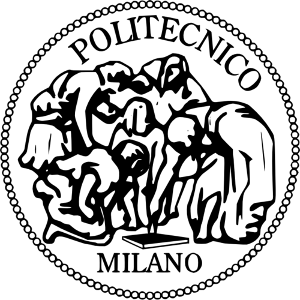
\includegraphics[width=3.7cm]{./pictures/logopm}
%	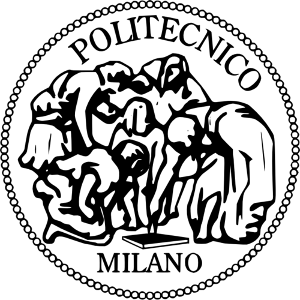
\psfig{file=./pictures/logopm.jpg,width=3.5cm}
    \end{center}
  \end{figure}
  \vspace*{0.3cm} \huge



  \textbf{Schnorr Signature: \\ Additivity and Multisignature}\\



%  \vspace*{.75truecm} \large
%  AI \& R Lab \\
%  Laboratorio di Intelligenza Artificiale \\
%  e Robotica del Politecnico di Milano
\end{center}
\vspace*{8.0cm} \large
\begin{flushleft}

\begin{tabular}{ll}
	Relatori:& Prof. Daniele Marazzina\\
	 & Prof. Ferdinando Ametrano\\
\end{tabular}


\end{flushleft}
\vspace*{1.5cm}
\begin{flushright}


  Tesi di Laurea di:\\ Chiara Lelli \\Matricola 830091


\end{flushright}
\vspace*{0.5cm}
\begin{center}



  Anno Accademico 2016-2017
\end{center} \clearpage
}

	\pagestyle{empty} \normalfont 
	\vspace{17cm}

%\large
\begin{flushright}
\itshape{ A Luca e i miei genitori \dots}
\end{flushright}


	\afterpage{\blankpage}

	\pagenumbering{Roman} \pagestyle{plain} 
\tableofcontents

	




	
	\listoffigures
	\listoftables
%	\listofalgorithms
%	\include{sommario}
	\newpage
\chapter*{Abstract}
\addcontentsline{toc}{chapter}{Abstract}
In 1991 on the \textit{Journal of Cryptology}, Claus Peter Schnorr published a paper titled \textit{"Efficient Signature Generation by Smart Cards"}, where he presented his idea for a new efficient signature scheme.\\
Even if it has so many interesting features and benefits, it has not been standardised yet. We present our implementation of \textit{Schnorr Signature} applied to Elliptic Curve Cryptography, which is based on the assumption of the Discrete Logarithm Problem.\\
Throughtout our dissertation, we explain our choices step by step and we illustrate the various properties of this signature, such as shortness, fast verification, but most of all \textit{additivity}. This one is not present in any other signature, and leads to a very important and innovative feature: \textit{multisignature}, a protocol through which a group of signers can generate a single joint signature on a common message.\\
We illustrate also our implementation of multisignature scheme and the several benefits brougth by this feature.\\
Finally, we introduce Elliptic Curve Digital Signature Algorithm, currently used in Bitcoin, showing how much improvements Schnorr Signature Algoritmh carries with it.
	
	\thispagestyle{plain} \cleardoublepage
	\afterpage{\blankpage}
	\renewcommand{\chaptermark}[1]{\markboth{\chaptername\ \thechapter.\ #1}{}} 
	\renewcommand{\sectionmark}[1]{\markright{\thesection.\ #1}}         
	\fancyhead[LE,RO]{\bfseries\thepage}    
	
	\fancyhead[RE]{\bfseries\leftmark}    
	\fancyhead[LO]{\bfseries\rightmark}     
	\renewcommand{\headrulewidth}{0.3pt} 
	
	\pagenumbering{arabic}
	\chapter{Introduction}
\label{Introduzione}

In this chapter, we illustrate a general overview of cryptography and digital signature and we present the main contribution of this work.
\section{General overview}
In \textit{Encyclop\ae dia Britannica\cite{EnBrit}}, Cryptography is defined as "the science of transforming information into a form that is impossible or infeasible to duplicate or undo without knowledge of a secret key". The first known evidence of the use of cryptography dates back to around 1900 BC in Egypt. We have to wait until 100 BC to see the first most famous cipher: Cesar Cipher. He used it to convey secret messages to his army generals. The key was to shift every letter by 3. The most famous example of cryptography is the cipher machine \textit{Enigma}, highly used by German forces during the Second World War.\\
\\
In 1976 Whitfield Diffie and Martin Hellman published "New Directions in Cryptography", introducing the idea of
public key cryptography. In fact, \textit{symmetric cryptography} has some shortcomings. The  secret key must be established trhough a secure channel and has to be known by only two people. Thus, if A wants to communicate through this system with several people, A has to store a large number of secret keys, one for each of the counterparts. There must be mutual trust between the parts and no one should want to cheat the other.\\
\\
This drawbacks have been overcomed through the introduction of the \textit{public key cryptography}, also known as \textit{asymmetric cryptography}. In this type of systems, the user has a key-pair: a \textit{public key} disclosed, and a \textit{private key} known only by the user. \\
The main uses of this system are:
\begin{itemize}
	\item \textit{public key encryption}: the message is encrypted using the recipient's public key and can be decrypted only by the owner of the corresponding private key.
	\item \textit{digital signature}: in this case the message is not encrypted, but it is signed using the sender's private key and can be verified by anyone using the corresponding public key.
\end{itemize} 
In this thesis, we focus on a specific digital signature: \textit{Schnorr Signature}. It was proposed in 1989 by Claus Pieter Schnorr, a German mathematician and cryptographer. It was published two years later and suddenly patented.\\
Even if it has always been known to be very simple, while other signatures such as DSA have been standardized, this has not happened to Schnorr signature because of the patent on it. Thus, when in 2005 the patent has expired, people have built on DSA rather than Schnorr signature.\\
\\
Actually there are some proposals for the implementation of this signature, but still no standard and no code to use it.
\section{Contributions}
This work provides an implementation of \textit{Schnorr Signature Algorithm} applied to Elliptic Curve Cryptography and \textit{Multisignature Protocol}. Since this signature has not been standardized yet, it is possible to find some ideas proposed by some researchers, but not a script on which the schemes are implemented. We chose to follow the guide line designed by Pieter Wuille, a very important Bitcoin Core developer. \\
\\
We start with an important overview of the mathematics necessary in order to deeply understand Elliptic Curve Cryptography and the assumptions on which it is based. Then we focus on \textit{Schnorr Signature}, starting from the analysis of the idea behind the algorithm, and going on presenting our implementation and explaining it step by step. A key point in our dissertation is the analysis of the benefits of SSA, among which the most important is: \textit{additivity}.\\ 
\\
This property is the basis of \textit{multisignature}, the main core of this dissertation. It is a protocol through which a group of signers can generate a single joint signature on a common message. We illustrate our implementation of this feature and we analyse it step by step.\\
\\
Finally, we present the Digital Signature Algorithm applied to an Elliptic Curve and compare it to ECSSA. We conclude explaining in details why ECSSA should replace ECDSA.

\section{Structure of the thesis} 
This work is organized as follows.
\begin{description}
	\item[Chapter 2] introduces the problem in mathemathical terms and it gives the necessary definitions on which we base our work.
	\item[Chapter 3] illustrates Schnorr Signature. Our algorithm is presented and analysed
	\item[Chapter 4] presents the most important feature of SSA: Multisignature. In this chapter, we show our implementation explaining it in every detail.
	\item[Chapter 5] illustrates the Digital Signature Algorithm and compares it to SSA 
	\item[Chapter 6] concludes the discussion with a summary of the results and suggests some possible future developments of this work.
\end{description}
	\chapter{State of the Art}
\label{capitolo2}


In this chapter, we present some basic notion and definition necessary to deeply understand how elliptic curve cryptography works.\\
We start with the mathematical foundations, from Modular Arithmetic to Groups and Finite fields. Then we go through an accurate analysis of Elliptic Curve and Hash functions to, finally, comprehend digital signatures.

\section{Mathematical Fundations}
Gauss used to say "\textit{Mathematics is the queen of the sciences, and number theory is the queen of mathematics}" because of its importance in the discipline. Number theory, as it is defined in \textit{Encyclop\ae dia Britannica\cite{EnBrit}}, is a branch of pure mathematics concerned with the properties of the positive integers. \\
It has applications to cryptography and cryptanalysis, particularly with regard to modular arithmetic and diophantine equations (i.e. \textit{elliptic curve}).
\subsection{Modular Arithmetic}
Modular Arithmetic can be informally called the "clock arithmetic". Indeed, the most familiar example of it is in the 12-hour clock, where the day is divided into two 12-hour periods. Here it is visible how numbers "wrap around" upon reaching the \textit{modulus} value, just like the hours of the day do in the clock.\\
For example, if it is 7:00 AM now, then 8 hours later what time will it be? Typically we would say 7 + 8 = 15, but in this case we will say 3:00 PM, because clock time "wraps around" every 12 hours. Thus, clock time is an example of \textit{modulus} 12.
\begin{figure}[H]
	\centering
	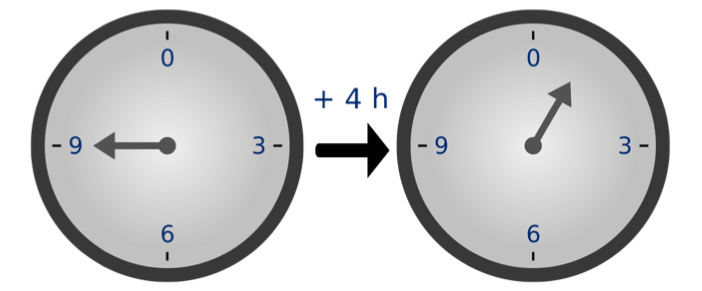
\includegraphics[width=.75\textwidth]{clock.png}
	\caption{Real-life example of modular arithmetic\cite{wiki}.}
	\label{img:clock}
\end{figure}

\begin{teorema}
	Given two integers $a$ and $b$, and a positive one $n$. $a$ and $b$ are said to be \textit{congruent modulo n}, if their difference $a-b$ is an integer multiple of $n$.\\
	The congruence relation is denoted 
	\begin{equation}
	a \equiv b\bmod n
	\end{equation}
\end{teorema}
The integers modulo $m$ are the possible remainders modulo $m$. They are denoted by $\mathbb{Z}_{m}$. The set of integers modulo $m$ is $\mathbb{Z}_{m}$=\{0, 1,$\dots$,m-1\}.

\paragraph{Properties}
Let $a_{1}, a_{2}, b_{1}$ and $b_{2}$ be integers such that $a_{1}\equiv b_{1}\bmod\ n$ and $a_{2}\equiv b_{2}\bmod\ n$. Thus:
\begin{equation}
	a_{1}+a_{2}\equiv b_{1}+b_{2}\bmod\ n
\end{equation}

\begin{equation}
	a_{1}-a_{2}\equiv b_{1}-b_{2}\bmod\ n
\end{equation}

\begin{equation}
	a_{1}a_{2}\equiv b_{1}b_{2}\bmod\ n
\end{equation}
these are, respectively, \textit{addition, subtraction} and \textit{multiplication}.
Moreover,given $a,b$:
\begin{equation}
	(a\bmod\ n)(b\bmod\ n)\equiv (ab)\bmod\ n
\end{equation}

\begin{equation}
	((a\bmod\ n)(b\bmod\ n))\bmod\ n\equiv (ab)\bmod\ n
\end{equation}

\subsection{Groups and Finite Fields}
Cryptography bases its basis also onto groups, rings and finite fields theory.

\begin{teorema}{\textbf{Group (G,*)}}\\
	A set G together with a binary operation $*$, that combines two elements $a$ and $b$ to form another element $a*b$, is a \textit{group} if it satisfies four requirements, known as the \textit{group axioms}:
	\begin{itemize}
		\item \textbf{Closure}: $\forall a,b \in G,\ a*b \in G$.
		\item \textbf{Associativity}: $\forall a,b,c \in G,\ (a*b)*c=a*(b*c)$.
		\item \textbf{Identity}: there exists an unique element $e \in G$ such that, $\forall a\in G$, $a*e=e*a=a$.
		\item \textbf{Invertibility}: $\forall a\in G$ there exists an element $b\in G$ such that, $a*b=b*a=e$.
	\end{itemize}
\end{teorema}

If $\forall a,b\in G$ $a*b=b*a$, $(G,*)$ is a \textit{commutative group}, also known as \textit{Abelian Group}.
\begin{example}
	Integers under addition $(\mathbb{Z},+)$ is an \textit{Abelian Group}; while integers under multiplication $(\mathbb{Z},\times)$ is not even a group.
\end{example}

\begin{example}
	For any modulus $p$ ([0,p-1],+) is a commutative group:
	\begin{itemize}
		\item $0$ is the \textit{identity} element 
		\item $\forall$ a, p-a is the \textit{inverse}
	\end{itemize}
\end{example}

\begin{example}
	For any prime number p ([1,p-1], $\times $) is a commutative group:
	\begin{itemize}
		\item 1 is the identity number
		\item $\forall a$ there exists its inverse, such that $ab\equiv$ 1 mod p	
	\end{itemize}
\end{example}

A group is called finite if it has a finite number of elements. The number of elements is called the \textit{order} of the group.\\

A group is \textit{cyclic} if its elements are \textit{powers} of a particoular one.\\
In this case, the element $g$ is the \textit{generator} of the group.

\begin{teorema}{\textbf{Ring (G,+,$\times$)}}\\
	A set G together with two binary operations (+, $\times$), is a ring if it satisfies the following requirements, the \textit{ring axioms}:
	\begin{itemize}
		\item (G,+) is an abelian group.
		\item (G,$\times$) is a \textit{semigroup}, which basically means that it satisfies the associativity property.
		\item $\times$ is \textit{distributive} with respect to +, it means that $\forall a,b,c \in G$:
		\begin{enumerate}
			\item $a\times (b+c)=(a\times b)+(a\times c)$.
			\item $(a+b)\times c=(a+c)\times (b+c)$.
		\end{enumerate}
	\end{itemize}
\end{teorema}

\begin{teorema}{\textbf{Field $\mathbb{F}$}}\\
	A field $\mathbb{F}$ is a ring such that the second operation satisfies all the group properties for all the elements but the identity element of the first operation.
\end{teorema}

A field which contains a finite number of elements is a \textit{finite field}.




\section{Elliptic Curve}
Now that we have given the preliminary definitions, we can introduce the theory of the Elliptic Curve, which is the basis of this thesis.
\begin{teorema}{(\textbf{Formal definition})}
	In mathematics, an elliptic curve is a plane algebraic curve defined in terms of the Weierstrass equation:
	\begin{equation}
	\label{eqn:EC}
	 y^{2}=x^{3}+ax+b
	\end{equation}
	that is non-singular; that is, it has no cusps or self-intersections.
\end{teorema}

Depending on the value of $a$ and $b$, elliptic curves may assume different shapes on the plane.

\begin{figure}[H]
	\centering
	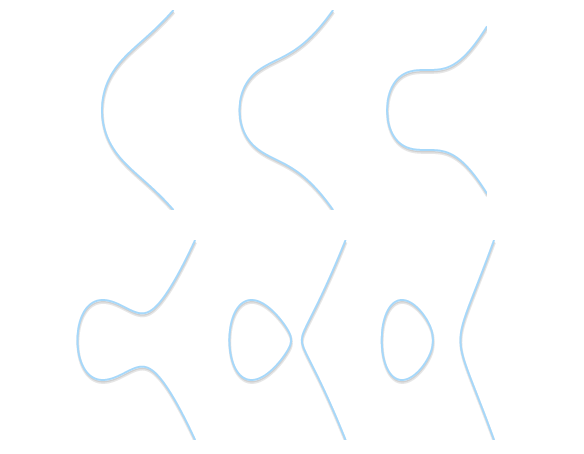
\includegraphics[width=.75\textwidth]{eccurves.png}
	\caption{Examples of elliptic curves\cite{graf}.}
	\label{img:ec_curves}
\end{figure}

The points of an elliptic curve together with the \textit{addition operation, +,} form an \textit{Abelian Group}, where:
\begin{itemize}
	\item \textbf{identity point}: the \textit{point at infinity} $\mathcal{O}$.
	\item \textbf{inverse} of the point $P$: its symmetric about the $x$-axis.
	\item \textbf{addition rule}: give three aligned, non-zero points over the EC $P,Q$ and $R$, $P+Q+R=0$.
\end{itemize}
As this is an abelian group, the addition becomes: $P+Q=-R$. So, in order to compute $P+Q$ you have to draw the line passing through $P$ and $Q$; $R$ is the third intersected point. The result of the addition operation is the inverse of $R$, $-R$.

\begin{figure}[H]
	\centering
	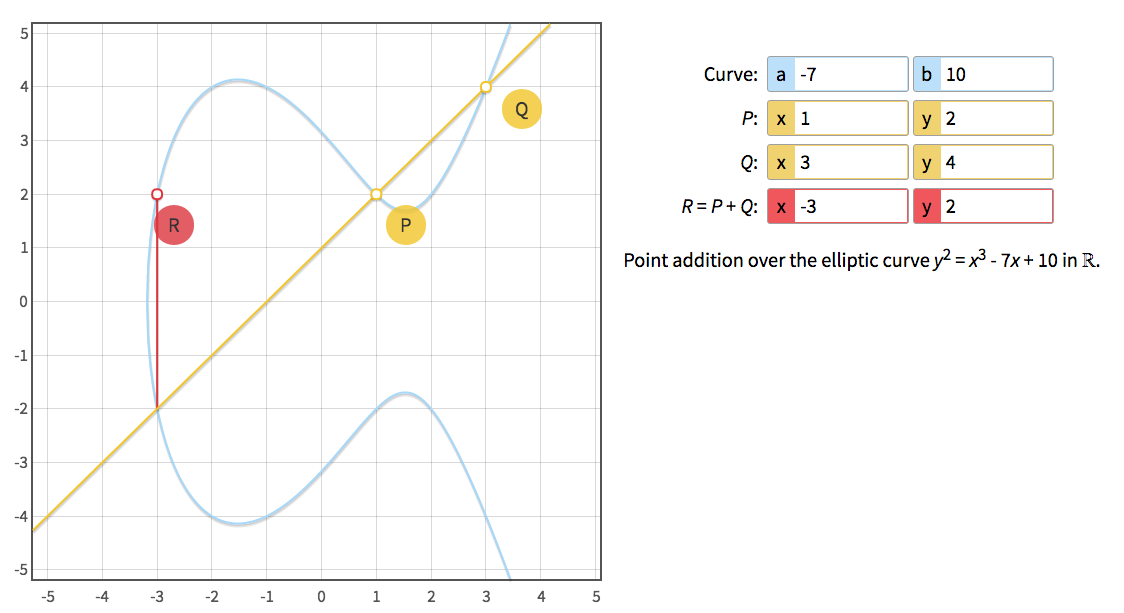
\includegraphics[width=.7\textwidth]{ec_somma.png}
	\caption{Addition\cite{graf}.}
	\label{img:ec sum}
\end{figure}
Formally, we should compute:
\begin{equation}
m=\frac{y_{P}-y_{Q}}{x_{P}-x_{Q}}
\end{equation}

\begin{equation}
x_{R}=m^{2}-x_{P}-x_{Q}
\end{equation}

\begin{equation}
y_{R}=y_{P}+m(x_{R}-x_{P})
\end{equation}

If $P=Q$, you have to draw the tangent to the curve in $Q$.

\begin{figure}[H]
	\centering
	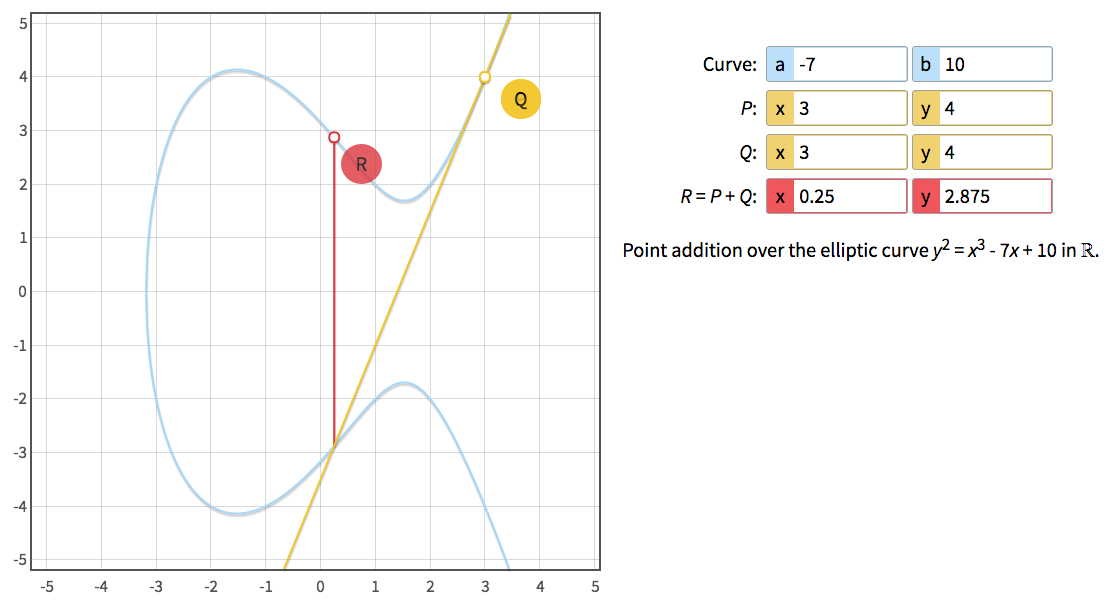
\includegraphics[width=.7\textwidth]{doubling.png}
	\caption{Point Doubling\cite{graf}.}
	\label{img:ec prod}
\end{figure}

If $P\neq Q$ but the line intersects only two points, then the line should be tanget to the curve. $R$ is the inverse of the point of tangency.

\subsection{Over a finite field}
Let \textit{E} be an elliptic curve over a finite field $\mathbb{F}_{p}$, where $p$ is a very high prime number, $p\neq 2,3$. Then, \textit{E} is described by the Equation \eqref{eqn:EC}, where $a,b \in \mathbb{F}_{p}$, such that $4a^{3}+27b^{2}\neq 0$.\\
The last requirement ensures that \textit{E} is non-singular, this means in particular that it is possible to compute the tangent in every point of the curve.\\
The of the \textit{rational points} in \textit{E} over $\mathbb{F}_{p}$, denoted by $E(\mathbb{F}_{p})$, is:
\begin{equation}
	E(\mathbb{F}_{p})=\{(x,y)\in \mathbb{F}_{p}^{2} :\ y^{2}\equiv x^{3}+ax+b (\bmod\ p),\ 4a^{3}+27b^{2}\not\equiv 0\ (\bmod\ p) \}\cup \{\mathcal{O}\}
\end{equation}

\begin{figure}[H]
	\centering
	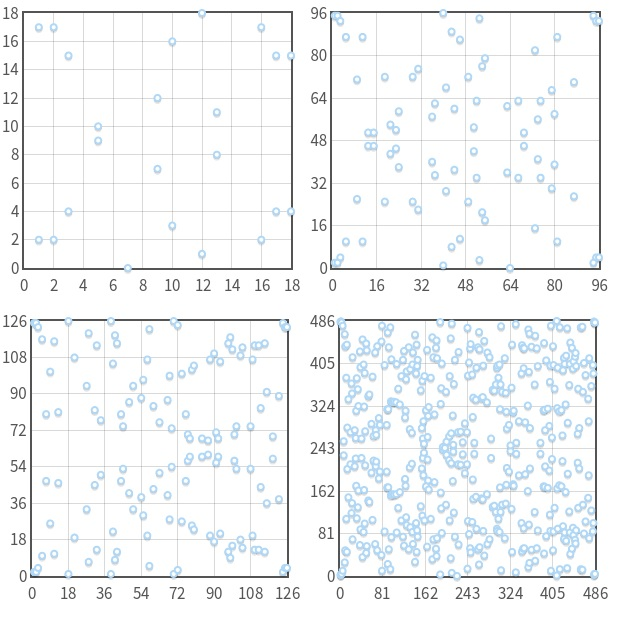
\includegraphics[width=.7\linewidth]{EC_ex.jpg}
	\caption{Examples of Elliptic Curve over Finite Fields\cite{graf}.}
\end{figure}
How does the addition operation changes in a finite field?\\
Informally, we can say that a line in $\mathbb{F}_{p}$ is the set of points $(x,y)$ which satisfy the equation $ax+by+c\equiv 0\ (\bmod\ p)$.
\begin{figure}[H]
	\centering
	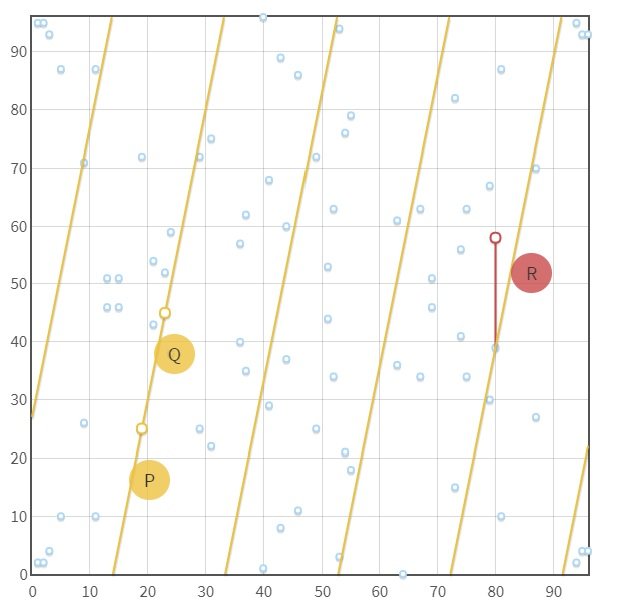
\includegraphics[width=.7\linewidth]{EC_aligned.jpg}
	\caption{Point addition on an EC over a Finite Field\cite{graf}.}
	\label{img:ec-ff}
\end{figure}
Note that the line $y\equiv 4x+83 (\bmod\ 127)$ that connects the points "repeats" itself in the plane.\\
Formally, we should compute:
\begin{equation}
m\equiv \frac{y_{P}-y_{Q}}{x_{P}-x_{Q}} (\bmod\ p),
\end{equation}

\begin{equation}
x_{R}\equiv m^{2}-x_{P}-x_{Q}\ (\bmod\ p),
\end{equation}

\begin{equation}
y_{R}\equiv y_{P}+m(x_{R}-x_{P})\ (\bmod\ p).
\end{equation}

\paragraph{Domain Parameters}
Elliptic curve domain parameters yield a set of information for communicating parties to identify a certain elliptic curve group for use in cryptography. The domain parameters comprise the finite field $\mathbb{F}_{p}$, the coefficients $a$ and $b$ of the $Weierstrass$ equation, a base point $G\in E(\mathbb{F}_{p})$, its order $n$,
and finally the cofactor $h=\frac{\#E(\mathbb{F}_{p})}{n}$. \\
The base point $G$ generates a cyclic subgroup of order $n$ in $E(\mathbb{F}_{p})$ denoted by $\langle{G}\rangle$, i.e.:
$\langle{G}\rangle= \{G, 2G,\dots, (n-1)G\} \cup {\mathcal{O}}$.

\begin{figure}[H]
	\centering
	\begin{tabular}{|l|l|}
		\hline
		\textbf{Parameter} & \textbf{Explanation}\\
		\hline
		\hline
		\textit{p} & A \textit{prime} number specifying the underlying field $\mathbb{F}_{p}$ \\
		\hline
		\textit{a} & The \textit{first} coefficient of Weierstrass equation \\
		\hline
		\textit{b} & The \textit{second} coefficient of Weierstrass equation \\
		\hline
		\textit{G} & The \textit{generator} point \\
		\hline
		\textit{n} & The \textit{order} of $G$ \\
		\hline
		\textit{h} & The \textit{cofactor} of $G$ \\
		\hline
	\end{tabular}
	\caption{Elliptic Curve domain parameters over $\mathbb{F}_{p}$\cite{ECC}.}
	\label{EC:dom par}
\end{figure}


\subsection{Bitcoin's Elliptic Curve}
Bitcoin uses the Koblitz curve \textit{secp256k1}, which has never been used before. It is characterised by the following parameters domain:
\begin{itemize}
	\item $p=FFFFFFFF\ FFFFFFFF\ FFFFFFFF\ FFFFFFFF\ FFFFFFFF\\ FFFFFFFF\ FFFFFFFE\ FFFFFC2F=2^{256}-2^{32}-2^{9}-2^{8}-2^{7}-2^{6}-2^{4}-1$
	\item $a=00000000\ 00000000\ 00000000\ 00000000\ 00000000\ 00000000\ 00000000\ 00000000$
	\item $b=00000000\ 00000000\ 00000000\ 00000000\ 00000000\ 00000000\ 00000000\ 00000007$
	\item $G=04\ 79BE667E\ F9DCBBAC\ 55A06295\ CE870B07\ 029BFCDB\ 2DCE28D9\\ 59F2815B\ 16F81798\ 483ADA77\ 26A3C465\ 5DA4FBFC\ 0E1108A8\ FD17B448\\ A6855419\ 9C47D08F\ FB10D4B8$ (uncompressed)
	\item $n=FFFFFFFF\ FFFFFFFF\ FFFFFFFF\ FFFFFFFE\ BAAEDCE6\\ AF48A03B\ BFD25E8C\ D0364141$
	\item $h=01$
\end{itemize}
So the EC over $\mathbb{F}_{p}$ is:\\ $E(\mathbb{F}_{p})=\{(x,y)\in \mathbb{F}_{p}^{2} :\ y^{2}\equiv x^{3}+7\ (\bmod\ p)\}\cup \{\mathcal{O}\}$.\\
Satoshi Nakamoto chose this curve because is the only one which was generated in a $non-random$ way, so it $30\%$ faster than the others. Moreover, it is defined over a ring, not over a binary Galois field.

\section{Discrete Logarithm}
The Elliptic Curve Cryptography, known as ECC, that is cryptography based on EC, is particularly interesting because it takes advantage of the fact that the Discrete Logarithm Problem (DLP) for EC is proven to be very "hard".
%Indeed it is simple, given $k$ and $P$, to compute $G=kP$
\begin{teorema}
	Let G be a cyclic group of order n with generator g. The discrete logarithm of $h\in G$ to the base g, denoted by $\log_{g} h$, is the unique integer k, $0\leq k \leq n-1$, such that $g^{k}=h$.\\
	Given g and h, the DLP is to find k.
\end{teorema}
The best known algorithms to break the elliptic curve discrete logarithm problem take steps proportional to $\sqrt{2^{n}} = 2^{\frac{n}{2}}$ , where $n$ is the number of bits of the key. \textit{secp256k1} uses 256 bit keys, so the number of steps needed to break it is $2^{128}$.

\section{Hash Function}
\begin{teorema}
	A hash function H is a one-way function that maps data of arbitrary size to a bit string of a fixed size, the hash value or digest.
\end{teorema}
Hash functions have a lot of useful applications in cryptography, such as digital signatures, message authentication, fingerprinting, and so forth.\\
In order to be suitable for cryptography, an hash function has to satisfy the following requirements:
\begin{enumerate}
	\item \textbf{Pre-image resistance}: given an hash value $h$ it is computationally infeasible to find $m$ such that $h=H(m)$.
	\item \textbf{Second pre-image resistance}: given an input $m_{1}$ it is computationally infeasible to find another input $m_{2}\neq m_{1}$, such that $H(m_{1})=H(m_{2})$
	\item \textbf{Collision resistance}: it is computationally infeasible to find two different inputs $m_{1}, m_{2}$, such that $H(m_{1})=H(m_{2})$.
\end{enumerate}

It is important to notice that \textit{Collision resistance} $\Rightarrow$ \textit{Second pre-image resistace}, but $\nRightarrow$ \textit{Pre-image resistance}.
\begin{example}
	One of the most diffused hash function is SHA-1 (produces a 160-bit (20-byte) hash value). It was designed by the United States National Security Agency, and is a U.S. Federal Information Processing Standard. Since 2005 SHA-1 has not been considered secure against well-funded opponents and, in 2017, CWI Amsterdam and Google announced they had performed a collision attack against SHA-1.\\
	So, it is not collision resistant $\Rightarrow$ it is not a good hash function.
\end{example}

Actually, Bitcoin uses SHA-256, which is one of the successor hash functions to SHA-1, and is one of the strongest hash functions currently available.
\paragraph{Properties} 
As we said before, the size of the possible hash values is smaller than the size of possible input data. Therefore, many input data points will share a single hash value output $\Rightarrow$ collisions do exist. But you have to try $2^{130}$ randomly chosen inputs in order to have $99.8 \% $ chance that two of them will collide. So, it is computationally unfeasible.\\
Hence, if we know $h(x) = h(y)$, it is safe to assume that $x= y$.
%\paragraph{Puzzle-friendliness}
%Given $x$ and a target set $Y$, to find $r$ from high min-entropy distribution such that $H(x|r)\in Y$, there is no solving strategy better than trying random values of $r$. (Brute force).\\
%Min-entropy measures how likely you are to guess a value on your first try. If this probability is $p$, then the min-entropy is defined as -$\log_{2} p$.\\
%For example, for a fair coin toss, you'd have $p = 0.5$, giving a min entropy of 1 bit. A uniformly random 256-bit string would have -$\log_{2} 2256 = 256$ bits of min entropy.

An important application of secure hashes is verification of message integrity. Determining whether any changes have been made to a message (or a file), for example, can be accomplished by comparing message digests calculated before, and after, transmission (or any other event).\\
For this reason, most digital signature algorithms only confirm the authenticity of a hashed digest of the message to be "signed". Verifying the authenticity of a hashed digest of the message is considered proof that the message itself is authentic.


\section{Elliptic Curve Cryptography}
In 1985, Neal Koblitz and Victor S. Miller independently proposed to use of the elliptic curves in cryptography. This brought to the birth of Elliptic-curve cryptography (ECC) which is a type of public-key cryptography based on the difficulty of computing discrete logarithms in the group of points on an elliptic curve defined over a finite field. 

\begin{teorema}{(\textbf{Public-key cryptography})}
	Public key cryptography, also known as asymmetric cryptography, is any cryptographic system that uses pairs of keys: \textit{public keys} which can be disclosed, and \textit{private keys} which must be known only by the owner.
\end{teorema}

\subsection{Key pair generation}
\textbf{Inputs:} The elliptic curve domain parameters \textit{(p, a , b, G, n, h)}. \\
\textbf{Actions:} The following actions are performed:

\hspace{1.1cm}
\begin{minipage}[l]{2\linewidth}
	\begin{enumerate}
		\item The \textbf{private key} is: $p=random({1, 2, \dots, n-1})$;
		\item The \textbf{public key} is: $P=p\times G$.\\
	\end{enumerate}
\end{minipage}
\textbf{Output:} $(p,P)$

$P$ is a point on the elliptic curve; while $p$ is an integer, the number of additive steps from the generator point $G$ to arrive at point $P$. \\
Here it becomes clear why it is fundamental that DLP is such a hard problem over elliptic curves! Indeed, the \textit{private key} must be secret, only the owner should know it; while the \textit{public key} can be known by everyone. That is also the reason why the \textit{prime} number of $E$ should be very high:\\
$p$ high $\implies n$ high $\implies$ it is unfeasible to know and try every single number in order to steal the \textit{private} key.
\subsection{Signature Protocol}
Until now, we have been focused on the mathematical structure that allows us to approach this type of cryptogrphy, but how does a signature algorithm work?\\
The scenario is the following: Alice wants to sign a message $m$ with her private key ($p_{A}$), and Bob wants to validate the signature using Alice's public key ($P_{A}$). Nobody but Alice should be able to produce valid signatures. Everyone should be able to check signatures. They are using the same domain parameters.\\
First, Alice generates her key pair and hashes the message, $h=H(m)$. With her private key, she generates her signature over $h$ and sends it to Bob.\\
This last computes $h$ and uses it, together with Alice's public key, in order to verify the validity of the received signature.\\
In the figure below it is represented this process.\\

\begin{figure}[H]
	\centering
	\renewcommand{\arraystretch}{2}
	\begin{tabular}{ccccc}
		\cline{2-2}\cline{4-4}
		 & \multicolumn{1}{|c|}{Message} &  &
		\multicolumn{1}{|c|}{Message}& \\
		\cline{2-2}\cline{4-4}
		 & $\Bigg\downarrow$ & & $\Bigg\downarrow$& \\
		\cline{2-2}\cline{4-4}
		 & \multicolumn{1}{|c|}{Hash Function} &  &
		\multicolumn{1}{|c|}{Hash Function}& \\
		\cline{2-2}\cline{4-4}
		 & $\Bigg\downarrow$ & & $\Bigg\downarrow$& \\
		\cline{2-2}\cline{4-4}
		 & \multicolumn{1}{|c|}{Message Digest} &  &
		\multicolumn{1}{|c|}{Message Digest}& \\
		\cline{2-2}\cline{4-4}
		 & $\Bigg\downarrow$ & & $\Bigg\downarrow$& \\
		\cline{2-2}\cline{4-4}
		$\xrightarrow{Private Key}$ & \multicolumn{1}{|c|}{Signature Generation} & $\xrightarrow[Signature]{Public Key}$&
		\multicolumn{1}{|c|}{Signature Verification}& $\xrightarrow{True/False}$\\
		\cline{2-2}\cline{4-4}
	\end{tabular}
\caption{Signature Process.}
\label{SigProt}
\end{figure}

	\chapter{Schnorr Signature Algorithm}
\label{capitolo3}
\thispagestyle{empty}

As we said in the introduction, Claus Peter Schnorr presented his idea in 1989, and he promptly patented it. Since the beginning of 2008, when the patent has expired, a lot of possible algorithms for the generation of Schnorr signature have been proposed, but still today there is no standard.\\
In this chapter, we present the one we think performs better: Schnorr Signature Algorithm over an Elliptic Curve.\\
First of all we illustrate the steps through which we can generate and verify this type of signature.
Then, we continue analyzing each codeline in order to deeply understand why we choose this implementation out of the various proposed by different developers.
Finally, we introduce the important benefits of this signature.



\section{Scheme}
Given an elliptic curve over a finite field $\mathbb{F} _{p}$, a user generates himself a private key \textit{p}, which is a random number $\in$ \{1, 2,\dots, \textit{n}-1\}, where \textit{n} is the group order. The corresponding public key \textit{P} is $\textit{p}\times G\bmod\ n$. \\
In order to sign a given message \textit{m}, the user has to choose another random number $k\in \{1, 2, \dots, \textit{n}-1\}$
, the \textit{ephemeral nonce}, and compute the \textit{Ephemeral key}, $\textit{K}= k \times G$.
\\
The signature consists of a pair of two integers $(r, s)$. The first is computed as the first coordinate of the Ephemeral
key; while the second integer, $s$, is 
computed as: 
\begin{equation}
\label{eqn:s}
s=k - h \times p\bmod\ n,
\end{equation}
where $h=H(m||r)$ is the hash value of the concatenation of the message and the first coordinate of the ephemeral key. \\
The pair $(r,s)$ is published as the signature.

A proceeds as follow to generate the EC-Schnorr signature $(r, s)$ on the message $m$.\\
\\
\textbf{Inputs:} The following informations are required as inputs.

\hspace{1.1cm}
\begin{minipage}[l]{2\linewidth}
\begin{enumerate}
	\item A's private key  \textit{$p_{A}$} and the elliptic curve domain parameters\\ \textit{(p, a , b, G, n, h)}.
	\item The message \textit{m} to be signed.\\
\end{enumerate}
\end{minipage}


\textbf{Actions:} The following actions are performed:

\hspace{1.2cm}
\begin{minipage}[l]{2\linewidth}
	\begin{enumerate}
		\item $\textit{k}=random({1, 2, \dots, n-1})$
		\item $K=k \times G$
		\item if $K$ is odd:
		\begin{itemize}
		      \item[a.] $k=n-k$
		      \item[b.] $K_{y}=p-K_{y}$
		\end{itemize}
		\item $r=K_{x}$
		\item $h=H(m||r)$\\
		If $h=0$ \ mod\ $n$ goto 1.
		\item $s=k - h \times p \bmod\ n$ \\
		If $s=0$ goto 1.
	\end{enumerate}
\end{minipage}

\textbf{Output:} The EC-Schnorr signature $(r, s)$ over $m$


\subsection{Verification}
The verification process is very important, because through it we can be sure that the message has been signed by the owner of the private key.\\
The protocol is simple, it consists of few steps:
\begin{itemize}
	\item Compute
	\begin{equation}
	\label{eqn:verif1}
	 V = K - h \times P;
	 \end{equation}
	\item If 
	\begin{equation}
	\label{eqn:verif2}
	V = s \times G,
	\end{equation} the signature is verified!
\end{itemize}

\paragraph{Proof of correctness}
We want to show that the verification protocol is mathematically correct.
\begin{proof}
	We can start analysing \eqref{eqn:verif2}. It is immediately visible that if we substitute \eqref{eqn:verif1} and \eqref{eqn:s} in it, we obtain
	\begin{equation}
	K - h \times P = (k - h\times p)\times G.
	\end{equation}
	Knowing that $K=k \times G$, 
	\begin{equation}
	(k - h\times p)\times G = (k - h\times p)\times G 
	\end{equation}
	
\end{proof}

Given a ECSSA signature $(r,s)$ over a message $m$, the verification procedure is the following: \\
\textbf{Inputs:} The following informations are required as inputs. 

\hspace{1.1cm}
\begin{minipage}[l]{2\linewidth}
	\begin{enumerate}
		\item A's authentic public key  $P_{A}$ and the elliptic curve domain \\parameters \textit{(p, a , b G, n, h)}.
		\item The message $m$ to be signed.
		\item The ECSSA signature $(r,s)$.\\
	\end{enumerate}
\end{minipage}
\textbf{Actions:} The following actions are performed:

\hspace{1.1cm}
\begin{minipage}[l]{2\linewidth}
	\begin{enumerate}
		\item if $s\geq order$: fail;
		\item if $r \geq prime$ number: fail;
		\item $h'= H(r||m)$;
		\item if $h'=0$ or $h'\geq order$: fail;
		\item $K'=h' \times P+s \times G$;
		\item if $K'_{y}$ is odd: fail;
		\item if $K'_{x} = r$ : \texttt{True}.\\
	\end{enumerate}
\end{minipage}
\textbf{Output:} \texttt{True}, if the signature is valid, and \texttt{False} otherwise




\section{Step by step analysis}

We continue our dissertation analysing each step, trying to highlight the reasons behind our decisions.\\
First of all it is very important that $k$ is always a random number, otherwise it is possible to find out the \textit{private key}.
\begin{example}
	Lets say that Alice wants to sign two messages, $m_{1}$ and $m_{2}$, using the same ephemeral nonce, k.\\ Everyone can see $(r_{1},s_{1})$, $(r_{2},s_{2})$, and the messages. So Bob, who wants to steal Alice's private key, is able to compute: \\
	$h_{1}=H(m_{1}||r_{1})$ and $h_{2}=H(m_{2}||r_{2})$.\\
	From \eqref{eqn:s}, Bob can easily trace back to $p$: 
	\begin{equation}
	\label{eqn:k}
	p= \frac{s_{2}-s_{1}}{h_{2}-h_{1}} \bmod\ n\\
	\end{equation}
\end{example}

In this simple way, everyone can find out Alice's private key and sign in lieu of her.\\
Going on into our analysis, why do we have to hash the message? \\
The reason behind this step has a practical nature: using a hash function $h$ we can reduce the amount of bytes; moreover, while the message can vary in its dimension, $h$ has a standard length.\\
%In his paper, Schnorr specified that the message should be hashed together with the $Ephimeral key$; we opted for the concatenation of $m$ and the $x$ coordinate of $K$.\\
The next step is the generation of the signature $s$. Schnorr inferred it from the ElGamal signature algorithm:
\begin{equation}
\label{eqn:ElGamal}
sk=m+xK (\bmod\ p-1),
\end{equation}
where $x$ is the \textit{private key}, $K$ is the $ephemeral\ key$ and the $k$ is the $ephemeral$ $nonce$.\\
Replacing $K$ by $h=H(m,K)$, $m$ can be eliminated. Another semplification comes from the replacements of $sk$ and $p-1$, respectively, by $s-k$ and the prime number $q$. This transforms \eqref{eqn:ElGamal} into:
\begin{equation}
s=k+hp (\bmod\ q),
\end{equation}
obtaining a much shorter signature.\\
This one is slightly different from the \eqref{eqn:s}, there is $-p$ in place of $p$. It would not be a problem except that, in this case, you should compute the $public\ key$ as $-p \times G$ instead of $p \times G$; but they require basically the same computational effort.\\
We now have understood why to hash the message, but why do we introduce the concatenation of message and $x$ coordinate of the \textit{ephemeral key}?\\
The reason is strictly linked to the most important property of this signature: \textit{linearity}.\\
As we will explain in the next section and in the next chapter, Schnorr signature is additive, so the signature of the sum is the sum of the signatures. This brings to amazing benefits, such as supporting naive multisignature, but it has some downside: Schnorr signature does not natively commit to the public key, which means that somebody can sign something using your key without knowing your private key. 
\begin{example}
	Let's say that Alice signs a transaction $T_{1}$ in Bitcoin system. Here, she computes her \textit{ephimeral nonce} $k_{1}$ deterministically. \footnote{Currently in Bitcoin, $k$ is generated through RFC6979 and it depends on $T$ and $p$.}
	$K_{1}=k_{1}\times G$, if $h_{1}=H(T_{1})$, then $s_{1}=k_{1}-p_{1}h_{1}$, so the signature is $(K_{1_{x}},s_{1})$.\\
	Now, Bob wants to sign the transaction $T_{2}$ ($h_{2}=H(T_{2})$) and is able to find out $k_{1}$, so
	\begin{equation*}
	h_{1}p_{1}=k_{1}-s_{1}.
	\end{equation*}
	He can decide that his private key is $p_{2}=\frac{p_{1}h_{1}}{h_{2}}$,
	\begin{equation*}
	s_{2}=k_{1}-h_{2}p_{2}	
	\end{equation*}
	$\implies s_{2}=k_{1}-p_{1}h_{1}=s_{1}$.\\
	In this way, Bob has obtained a valid signature $(K_{2_{x}},s_{2})$ identical to Alice's one and they are absolutely valid!
\end{example}

The last step is the output of the algorithm: $(K_{x},s)$.
Why do we use only the $x$ coordinate of the $Ephemeral\ key$ to sign the message? Why not adhere to Schnorr's paper?\\
Indeed, he thought about a different output: $(h,s)$, which occupies three-quarters of ours' space.\\
We chose $K_{x}$ instead of $h$ because otherwise it would not have been possible to make such an important processesas the \textit{key recovery}.

\begin{teorema}[\textbf{Key Recovery}]
	The Key recovery is the process through which is possible to trace back to a public key starting from one coordinate.
\end{teorema}

This process is very important, because it permits everyone to control the validity of the signature.\\
We could not have used the $y$ coordinate instead of the $x$ one, because the key recovery would require a higher computational effort. Moreover, there would be three $x$ coordinates among which we should find our key recovered rather than the two $y$ coordinates.\\
We obtain a 64-bytes signature:
\begin{itemize}
	\item a 32-byte integer $K_{x}$
	\item a 32-byte integer $s$ \\
\end{itemize}


\begin{figure}[H]
	\centering
	\renewcommand{\arraystretch}{2}
	\begin{tabular}{l|clcc}
		\textbf{Scheme} & \textbf{Public key} & \textbf{First component} & \textbf{Second component} & \textbf{Signature size}\\
		\hline
		[Sc91] & $-p \times G$ & $H(m,K)$ & $k+p h$ & $b+2b$\\
		EC-SDSA & $-p \times G$ & $H(K_{x}||K_{y}||m)$ & $k+p h$ & $2b+2b$ \\
		EC-SDSA-opt & $-p \times G$ & $H(K_{x}||m)$ & $k+p h$ & $2b+2b$ \\
		EC-FSDSA & $-p \times G$ & $K_{x}||K_{y}$ & $k+p h$ & $4b+2b$ \\
		EC-Schnorr & $p \times G$ & $H(K_{x}||m)$ & $k-p h$ & $2b+2b$ \\
		\rowcolor{yellow}
		EC-SSA & $p \times G$ & $K_{x}$ & $k-p h$ & $2b+2b$ \\
	\end{tabular}
	\caption{Characteristics of the proposed schemes.}
	\label{tabsig}
\end{figure}

In the table above are reported the different schemes among which we chose ours.\\
$[$Sc91$]$ is the one that most conforms to Schnorr's paper, and has the lowest signature's size: $b+2b$.\\
The following three schemes are an alteration of the EC-DSA, which is the current signature algorithm that is used by Bitcoin. (We will discuss about it in the fifth chapter.)\\
We rejected the first five ides because the first component does not allow the key recovery. In particular, the concatenation of the coordinates of the \textit{Ephemeral key} can be either a component of a point over the eliptic curve or not, so it is unusable; while the other schemes have an hash value as firts component, so no one besides \textit{ECSSA} supports the key recovery.\\
Moreover, EC-FSDSA has a very big signature.\\
So, currently the best possible scheme is EC-SSA.
\section{Benefits}

Here we want to highlight some feature of this signature. \\
The main reason behind the hype around Schnorr signature is the \textbf{additivity}. \\
What is it? And what does it involve?\\
This allows us to sum up two signatures creating just one valid signature.\\
Consequently, it brings to Multisignature, which we will thoroughly discuss in the following chapter.\\

%Examining our algorithm in depth, it is visible that excluding 

The \textit{non-malleability} is another important feature of this signature.

\begin{teorema}
	A signature scheme is malleable — alternatively, homomorphic— if, given a signature s on a message m, one can efficiently derive a signature s' on a message m' = T(m) for an allowed transformation T.
\end{teorema}

Consequently, if a signature scheme is non-malleable, a third party that does not have access to private key can not modify the signature without invalidating it.

Another important benefit of our choice is the possibility to implement \textit{Batch validation}.
\begin{teorema}[\textbf{Batch validation of signatures}]
	Let l be the security parameter. Suppose (Gen,Sign,Verify) is a signature scheme, $k, n \in poly(l)$, and $(pk_{1},sk_{1}), \dots, (pk_{n},sk_{n})$ are generated indipendently according to Gen($1^{l}$). Let PK=${pk_{1},\dots,pk_{n}}$. Then we call Batch a batch verification algorithm when the following conditions hold:
	\begin{itemize}
		\item If $pk_{t_{i}} \in PK$ and Verify($pk_{t_{i}},m_{i},\sigma_{i}$)=1 for all $i \in [1 \dots n]$, then Batch($(pk_{t_{1}},m_{1},\sigma_{1}),\dots, (pk_{t_{n}},m_{n},\sigma_{n})$)=1.
		\item If $pk_{t_{i}} \in PK$ and Verify($pk_{t_{i}},m_{i},\sigma_{i}$)=0 for some $i \in [1 \dots n]$, then Batch($(pk_{t_{1}},m_{1},\sigma_{1}),\dots, (pk_{t_{n}},m_{n},\sigma_{n})$)=0.
	\end{itemize}
\end{teorema}
The idea behind Batch validation is that you can have multiple sets of combinations of keys and messages and you can verify them all at once.


%non-malleability
%security proof


\noindent 
	\chapter{Multisignature}
\label{capitolo4}
In this chapter we want to analyse the most important feature of Schnorr Signature: multisignature.\\
More often than not, $n$ people are asked to sign the same document or transaction. In these cases, it is used a \textit{multisignature} scheme. It is supported by also others digital signatures, but the amazing thing of Schnorr Signature is that it supports a \textit{native multisignature} scheme.\\
Firstly, we focus on \textit{additivity}, which is the property that leads to the main core of our work.\\
We continue showing the scheme that we have implemented and, finally, we analyse the reasons behind every choice taken.\\

\section{Key Aggregation}
The biggest innovation brought by Schnorr signature is the \textit{Key Aggregation}, which, according to \cite{MuSig}, means that the joint signature can be verified exactly as a standard Schnorr signature with respect to a single ``aggregated" public key which can be computed from the individual public keys of the signers.\\
Key aggregation is closely related to \textit{additivity}.
\subsection{Additivity}
\textit{Additivity} is a very important property of Schnorr signature.
In \cite{NovAdd}, Greg Friedman introduces the connection between additivity and additive signature: given two manifolds $M_{1}$, $M_{2}$ glued together along a common boundary. \textit{Additivity} holds when the signature is additive with respect to this decomposition.\\
In order to understand this statement, Friedman introduces bilinear forms. In particular, given a bilinear form on finite dimensional $\mathbb{R}$-vector spaces
\begin{equation*}
\phi:V \otimes V \to \mathbb{R},
\end{equation*}

it is symmetric if $\phi(v,u)=\phi(u,v)$ $\forall v,u \in V$. The matrix representation is $M_{ij}=\phi (e_{i},e_{j})$.\\
Two considerations the author does in the paper are very important for our implementation:
\begin{quote}
	\begin{itemize}
		\item $(V_{1},\phi_{1}),\ (V_{2},\phi_{2})$ produces $\phi_{1} \boxplus \phi_{2}$ on $ V_{1}\oplus V_{2}$:
		\[ 
		\begin{pmatrix}
			 \phi _{1}  & 0\\
			0 &  \phi_{2} 
		\end{pmatrix} 
		\] \footnote{$\boxplus$ symbolises the \textit{free additive convolution}}
		The signature of the sum is the sum of the signatures.
		\item On $V_{1} \bigotimes V_{2}$, there is a natural form. The signature $\sigma(\phi_{1}\otimes \phi_{2})= \sigma(\phi_{1}) \sigma(\phi_{2})$\footnote{$\otimes$ symbolises the \textit{tensor product}}
	\end{itemize}
\end{quote}

Both the considerations have an important implication:\\
since the elliptic curve is a finite dimensional $\mathbb{R}$-vector space, Schnorr signature is additive.\\
We have taken advantage of this property and we have implemented a \textit{multisignature} scheme.

\section{Scheme}
This scheme consists of 3 stages and one preparatory step (Stage 0).
\paragraph{Stage 0} 
Given the elliptic curve domain parameters \textit{($\overline{p}$, a, b, G, n, h)} and The message $m$ to be signed, each user $i$ has to generate his key pair $(p_{i},P_{i})$.\\

\textbf{Inputs:} Every signer $i$ has to provide his public key $P_{i}$.

\textbf{Actions:} The following actions are performed:

\hspace{1.2cm}
\begin{minipage}[l]{2\linewidth}
	\begin{enumerate}
		\item The hash value of $P_{i}$, $h'_{i}=H(P_{i})$.
		\item $P_{All}=\sum_{i} h'_{i}\times P_{i}.$
	\end{enumerate}
\end{minipage}

\textbf{Output:} $P_{All}$.

\paragraph{Stage 1}

Every signer $i$ has to choose his \textit{ephemeral private key} $k_{i}$, compute the \textit{Ephemeral public key} $K_{i}$ and give to the other signers the $x$ coordinate $K_{x_{i}}$

\paragraph{Stage 2}
In this stage everyone computes his own signature $s_{i}$ and the \textit{Ephemeral public key} related to the \textit{multisignature}. Everyone has to follow this process.\\
\textbf{Inputs:} Every signer $i$ has the following informations as inputs.

\hspace{1.1cm}
\begin{minipage}[l]{2\linewidth}
	\begin{enumerate}
		\item The message $m$.
		\item His private key $p_{i}$.
		\item His \textit{ephemeral key pair} ($k_{i}, K_{i}$).
		\item The $x$ coordinate of the \textit{ephemeral public key} of the other signers, $K_{x_{j}},\ \forall j\neq i$
	\end{enumerate}
\end{minipage}


\textbf{Actions:} Every user, indipendently from the others, performs the following instructions:

\hspace{1.2cm}
\begin{minipage}[l]{2\linewidth}
	\begin{enumerate}
		\item $p'_{i}= p_{i}\times h'_{i}$
		\item if $K_{i}$ is odd:
		\begin{itemize}
			\item[a.] $k_{i}=n-k_{i}$
			\item[b.] $K_{y_{i}}=\overline{p}-K_{y_{i}}$
		\end{itemize}
		\item $\forall j\neq i$, $i$ recovers $K_{j}$
		\item $K_{All_{i}}=\sum_{j\neq i}\ {K_{j}}+K_{i}$
		\item if $K_{All_{i}}$ is odd:
		\begin{itemize}
			\item[a.] $k_{i}=n-k_{i}$
			\item[b.] $K_{All_{i_{y}}}=\overline{p}-K_{All_{i_{y}}}$
		\end{itemize}
		\item $h_{i}=H(m||K_{All_{i_{x}}})$\\
		If $h_{i}=0$ \ mod\ $n$ goto 1.
		\item $s_{i}=k_{i} - h_{i} \times p'_{i} \bmod\ n$ \\
		If $s_{i}=0$ goto 1.
	\end{enumerate}
\end{minipage}

\textbf{Output:} $(K_{All_{i_{x}}}, s_{i})$
\paragraph{Stage 3}
In this stage, takes place the combination of the previous outputs, in order to compute the final signature.\\
\textbf{Inputs:} Every signer $i$ has to provide the following informations as inputs.

\hspace{1.1cm}
\begin{minipage}[l]{2\linewidth}
	\begin{enumerate}
		\item $K_{All_{i_{x}}}$.
		\item His signature $s_{i}$.\\
	\end{enumerate}
\end{minipage}


\textbf{Actions:} The following instructions are performed:

\hspace{1.2cm}
\begin{minipage}[l]{2\linewidth}
	\begin{enumerate}
		\item if $K_{All_{i_{x}}}=K_{All_{j_{x}}}$ $\forall i,j$: $K_{All_{x}}= K_{All_{i_{x}}}$.
		\item else: fail.
		\item $s_{All}=\sum_{i}{s_{i}}$.\\
		If $s_{All}=0$ or $s_{All}\geq n$: fail.
	\end{enumerate}
\end{minipage}

\textbf{Output:} The Multisignature $(K_{All_{x}}, s_{All})$ over $m$

We want to highlight that along the process the signers have to communicate each other some informations, such as between stage 1 and 2: among the inputs of stage 2 there are the $x$ coordinate of the \textit{ephemeral public key} of the other cosigners.
\subsection{Verification}
Through the process explained above, we have obtained one signature in place of $N$ single signatures. The most fascinating property is that this signature acts as a single one, so the verification process is the same presented in Chapter 3, but in this case the inputs are slightly different: $P_{All}$ in place of the single $P_{i}$.
\begin{itemize}
	\item Compute
	\begin{equation}
	\label{eqn:verifM1}
	V = K_{All} - h \times P_{All};
	\end{equation}
	\item If 
	\begin{equation}
	\label{eqn:verifM2}
	V = s_{All} \times G,
	\end{equation} the signature is verified!
\end{itemize}

\paragraph{Proof of correctness}
We want to show that the verification protocol is mathematically correct.
\begin{proof}
	Knowing that $s_{All}=\sum_{i}{s_{i}}$, it is immediately visible that if we substitute \eqref{eqn:verifM1} and \eqref{eqn:s} in \eqref{eqn:verifM2}, we obtain
	\begin{equation}
	\sum_{i} {K_{i} - h_{i} \times (P_{i}\times h'_{i})} =\sum_{i} (k_{i} - h_{i}\times p'_{i})\times G.
	\end{equation}
	But $K_{i}=k_{i} \times G$, and $h_{i}=h\ \forall i$ because $h_{i}=H(m||K_{All_x})$. Moreover, $p'_{i}= p_{i}\times h'_{i}$, where $h'_{i}=H(P_{i})$. Thus,
	\begin{equation}
	\sum_{i} {k_{i} \times G - h \times (P_{i}\times h'_{i})} =\sum_{i} (k_{i} - h\times p_{i}\times h'_{i})\times G.
	\end{equation}
	
\end{proof}


\section{Step by step analysis}
Now we want to highlight the purpose of each step delineated above.\\
We should start with stage 1, where signers have to communicate the $x$ coordinate of their \textit{Ephemeral public key}, $K_{x}$. This step is fundamental because in stage 2 everyone has to recover the \textit{ephemeral public keys} of the cosigners in order to compute $K_{All_{i}}$. Otherwise it would not be possible to generate a key aggregation using the additivity property. Actually, the users could send their entire $K_{i}$, but it would duplicate the cost of communication obtaining the same result. Not by chance, we ask to control the parity of their own key before sending it: in this way we know that every key is positive.\\
Going on in the second stage, the signatures are generated following the usual scheme.\\
The last steps we should focus on are:
\begin{enumerate}
	\item $P_{All}=\sum_{i} h_{i}\times P_{i}$
	\item $p_{i}=p_{i}\times h_{i}$,
\end{enumerate}
where $h_{i}=H(P_{i})$.\\
In the original idea there were not the $h_{i}$, but they are fundamental. Without them the \textit{Rogue key attack} would be possible, see next section.
\subsection{Cancellation attack}
The \textit{Rogue Key attack}, also known as \textit{Cancellation attack}, is an attack made by malicious users who manipulate public keys in order to produce forgeries of the set of public keys.\\
Since everyone knows the various public keys $P_{i}$ and $P_{All}=\sum_{i} P_{i}$, the corrupted signers can easly compute their $P_{i}$ as a combination of all the public keys so that $P_{All}=\sum_{j} P_{j}$ where $j$ are the malicious signers.
\begin{example}
	Let Alice and Bob want to sign the same message $m$ through the \textit{multisignature} scheme where $P_{All}=\sum_{i} P_{i}$.\\
	Alice is honest, while Bob wants to have the control of the signature all alone.\\
	Bob can pretend that his public key is $P'_{B}=P_{B}-P_{A}$; it is important to highlight that he can compute it because $P_{A}$ is known. \\
	$\implies P_{All}=P'_{B}+P_{A}=P_{B}-P_{A}+P_{A}=P_{B}$\\
	The signature is valid and the verifiers are not able to demonstrate that Bob has ripped off Alice and $P'_{B}$ is not his real public key.
\end{example}
This type of attacks was the reason why the first proposals failed and were abandoned. The first solution to this problem came from Micali, Ohta, and Reyzin in 2001 \cite{MOR}, but it was based on an interactive key generation protocol.\\
Another way to prevent Rogue-key attacks is to require the proof of knowledge of the secret key during public key registration, idea proposed by Thomas Ristenpart and Scott Yilek in their paper published in 2007 \cite{RY}.\\
Both the solutions were highly expensive. We implemented the idea explained in \cite{MuSig}, because it does not require additional interactions between the signers, much more cheaper than the previouse ideas.
\section{Benefits}
We have analyzed \textit{multisignature} in every step, but why have we implemented it?\\
This scheme allows us to save a lot of space, because in place of $n$ signatures we end up with only one!\\
This is fundamental, for example, in Bitcoin system. Bitcoin \cite{Nakamoto} is a p2p electronic cash system in which all participants (are able to) validate transactions. These transactions consist of outputs, which have a verification key and amount, and inputs which are references to outputs of earlier transactions not spent yet (known as UTXOs). Each input contains a signature. In fact, some outputs even require multiple signatures to be spent. Transactions spending such an output are often referred to as $m$-of-$n$ multisignature transactions, and the current implementation corresponds to the concatenation of the individual signatures. For each transaction are required from one to $m$ signatures. These transactions are stored in a distributed ledger, known as blockchain, composed by connected blocks where the transactions are stuffed into.\\
It is obvious that through a \textit{multisignature} scheme, the signature sizes would be lowered to the standard single signature of 64 bytes, regardless of the number of cosigners. Consequently, the transaction's size would diminish lowering the blocks' weight.\\
In the figure below it is represented the actual blockchain size and the one that it would have had if there had been a multisignature scheme since 2008.
\begin{figure}[H]
	\centering
	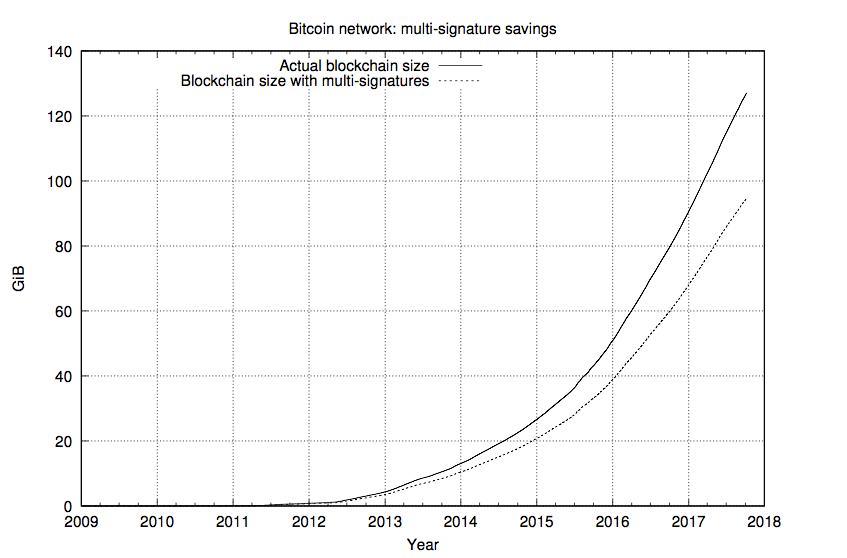
\includegraphics[width=.85\textwidth]{BlockchainMusig.png}
	\caption{Size of the Bitcoin blockchain with and without multi-signatures.}
	\label{img:BlockchainMusig}
\end{figure}
	\chapter{DSA vs SSA}
\label{capitolo5}

In this chapter, we introduce the Digital Signature Algorithm, which is the current signature used in Bitcoin. \\
We analyze the algorithm and we compare it with Schnorr Signature Algorithm.



\section{Digital Signature Algorithm}
Proposed in August 1991 by the U.S. National Institute of Standards and Technology (NIST) and become a U.S Federal Information Processing Standard in 1993, DSA was the first signature scheme  accepted legally by the U.S. government \cite{ECDSA}.\\
Particularly interesting is the application of DSA to Elliptic Curve Cryptography: ECDSA.\\
ECDSA works in the group of elliptic curve $E(Z_{p})$. In the early 00s it has been standardized by many standard committees such as ISO, ANSI, IEEE and FIPS. So, when Satoshy Nakamoto had to decide which standardized signature algorithm to adopt in Bitcoin, ECDSA was the best in circulation. In facts, it has some downsides that, as we are going to show you, could be solved adopting ECSSA.
\subsection{Scheme}
Given an elliptic curve over a finite field $\mathbb{F} _{p}$, a user generates himself a private key \textit{p}, which is a random number $\in$ \{1, 2,\dots, \textit{n}-1\}, where \textit{n} is the group order. The corresponding public key \textit{P} is $\textit{p}\times G\bmod\ n$. \\
In order to sign a given message \textit{m}, the user has to choose another random number \textit{k}%$\in$ \{1, 2, \dots, \textit{n}-1\}
, the \textit{ephemeral nounce}, and compute the \textit{Ephemeral key}, $\textit{K}= k \times G$.
\\
The signature consists of a pair of two integers $(x_{K}, s)$. The first is computed as the first coordinate of the Ephemeral
key; while the second integer, s, is computed as: 
\begin{equation}
\label{eqn:s2}
s=(h - x_{K} \times p) k^{-1}\bmod\ n
\end{equation}
where $h=H(m)$ is the hash value of the message. \\
The pair $(x_{K},s)$ is published as the signature.\\

A proceeds as follow to generate the ECDSA signature $(x_{K}, s)$ on the message \textit{m}.\\
\\
\textbf{Inputs:} The following informations are required as inputs.

\hspace{1.1cm}
\begin{minipage}[l]{2\linewidth}
	\begin{enumerate}
		\item A's private key  \textit{$p_{A}$} and the elliptic curve domain parameters\\ \textit{(p, a , b, G, n, h)}.
		\item The message \textit{m} to be signed.\\
	\end{enumerate}
\end{minipage}


\textbf{Actions:} The following actions are performed:

\hspace{1.2cm}
\begin{minipage}[l]{2\linewidth}
	\begin{enumerate}
		\item $\textit{k}=random({1, 2, \dots, n-1})$
		\item $K=k \times G$
		%\item $x_{K}=K_{x} \bmod\ n$
		\item $h=H(m)$\\
		If $h=0$ \ mod\ $n$ goto 1.
		\item $s=(h+x_{K}\times p)k^{-1}\bmod\ n$ \\
		If $s=0$ goto 1.
	\end{enumerate}
\end{minipage}

\textbf{Output:} The ECDSA signature $(x_{K}, s)$ over $m$


\subsection{Verification}
The verification process is very important, because through it we can be sure that the message has been signed by the owner of the private key.\\
The protocol consists of the following steps:
\begin{itemize}
	\item Compute:
	\begin{enumerate}
		\item \begin{equation}
			  \label{eqn:verifDSA1}
			  u = hs^{-1} \bmod\ n
			  \end{equation}
		\item \begin{equation}
			  \label{eqn:verifDSA2}
			  v = x_{K}s^{-1} \bmod\ n
			  \end{equation}
		\item \begin{equation}
			  \label{eqn:verifDSA3}
			  (x,y)=u\times G+ v\times P
			  \end{equation}
	 \end{enumerate}
 	\item If:
 	\begin{equation}
 	\label{eqn:verifDSA4}
 	x=x_{K}\bmod\ n
 	\end{equation} the signature is verified!
\end{itemize}

\paragraph{Proof of correctness}
We want to show that the verification protocol is mathematically correct.
\begin{proof}
	We can start noticing that \eqref{eqn:verifDSA4} is true if 
	\begin{equation}
	u\times G+ v\times P=K
	\end{equation}
	Since $P$ is the public key and $K$ is the ephemeral key:
	\begin{equation}
	(u+vp)\times G= k\times G
	\end{equation}
	Considering \eqref{eqn:verifDSA1} and \eqref{eqn:verifDSA2},
	\begin{equation}
	(hs^{-1}+x_{K}s^{-1}p)\times G= k\times G
	\end{equation}
	\begin{equation}
	(h+x_{K}p)s^{-1}\times G= k\times G
	\end{equation}
	Since $s$ is the signature,
	\begin{equation}
	(h+x_{K}p)(h+x_{K}p)^{-1}k\times G= k\times G
	\end{equation}
	$\implies k\times G=k\times G$ identity.
\end{proof}

Given a ECDSA signature $(x_{K},s)$ over a message $m$, the verification procedure is the following: \\
\textbf{Inputs:} The following informations are required as inputs. 

\hspace{1.1cm}
\begin{minipage}[l]{2\linewidth}
	\begin{enumerate}
		\item A's authentic public key  \textit{$P$} and the elliptic curve domain \\parameters \textit{(p, a , b G, n, h)}.
		\item The message \textit{m} to be signed.
		\item The ECDSA signature $(x_{K},s)$.\\
	\end{enumerate}
\end{minipage}
\textbf{Actions:} The following actions are performed:

\hspace{1.1cm}
\begin{minipage}[l]{2\linewidth}
	\begin{enumerate}
		\item if $s\geq order$: fail;
		\item if $x_{K} \geq prime$ number: fail;
		\item $v=x_{K}s^{-1} \bmod\ n$;
		\item $h'= H(m)$;
		\item if $h'\neq 0$ or $h'<order$:
		\begin{itemize}
			\item $u=h' s^{-1} \bmod\ n$;
			\item $(K'=u\times G + v\times P) \bmod\ n$;
		\end{itemize}
		\item else:
		\begin{itemize}
			\item $K'=v$
		\end{itemize}
		\item if $K'_{x} = x_{K}$ : \texttt{True}.\\
	\end{enumerate}
\end{minipage}
\textbf{Output:} \texttt{True}, if the signature is valid, and \texttt{False} otherwise


\section{Comparison}
Here we want to compare the scheme we propose to the one currently used in Bitcoin: ECSSA vs ECDSA.\\
We can start analysing \eqref{eqn:s} and \eqref{eqn:s2}, the generation of $s$:\\
they are both quite simple, the second requires a little bit more effort because it uses the multiplication by the inverse of $k$; anyway, the signature is a couple of integer. They differ in the use of the hash function:\\
in Schnorr, as we have demonstrated in \textit{Chapter \eqref{capitolo3}}, it must be $h=H(m||K_{x})$; while in ECDSA, it can easily be $h=H(m)$. This is because of the linearity, a property that the latter does not have. ECDSA, indeed, is not additive. Why?\\
The explanation lies in the  fact that ECDSA works with just the $x$-coordinate of the $Ephemeral\ key$, while Schnorr uses directly the points, so the latter exploits the $shifting\ property$:
\begin{teorema}{(\textbf{Shifting Property})}
	Let $P$ be a point on an Elliptic Curve with gerator $G$, $e$ be an integer, then:
	\begin{equation*}
	Q=P+e\times G
	\end{equation*}
	is an EC point. Moreover if $P = x \times G$ then $Q=(x+e) \times G$.
\end{teorema}
Operating with only one coordinate it is not possible to use this property, because:\\
$P_{x}+G_{x}=Q_{x} \nRightarrow P+G=Q$.\\
Looking at the left side, $Q_{x}$ could be the coordinate of an EC point, but it could also not be in the curve: we are not in a \textit{Cartesian plane}!\\
Indeed, Schnorr signature supports multisignature, while it is not possible to implement such a scheme in DSA. So, using the former there would be a considerable save of space! (\textit{see figure \eqref{img:BlockchainMusig}})\\
Moreover, currently it is used the DER encoding, which adds 6 bytes in each signature, and it is composed by:
\begin{itemize}
	\item $0x30$ to indicate the a DER encoded signature follows
	\item 1 byte for length of signature
	\item $0x02$ to indicate the a integer follows
	\item 1 byte for length of $x_{K}$
\end{itemize}
This means that the length of the signatures can vary. In our scheme it is not used and the length is fixed.\\
Schnorr signature saves up not only space, but also time.
Looking at the \textit{verification} process, indeed, in Schnorr is faster and simpler than in DSA. 
In this contex, it is important to remind what we said in \textit{Chapter \eqref{capitolo3}}, which is that SSA supports \textit{Batch Validation}. It is an amazing feature, because it permits to verify at the same time a set of signatures all together.\\
\\
Furthermore, DSA has some others drawbacks, such as \textit{mellability}.\\
So, for example, if $(x_{K},s)$ is a valid signature of $h$, also $(x_{K},n-s)$, where $n$ is the $order$, is a valid signature adn everyone can use it.\\
This cannot happen with SSA.\\


	\chapter{Conclusions and Future Work}
\label{capitolo6}


\section{Conclusions}
Throughout this dissertation we have analysed \textit{Schnorr Signature}, a digital signature proposed in 1989 by Schnorr, a German mathematician and cryptography. It has been particularly in the spotlight during the last few years, due to its properties, benefits and features.\\
Firstly, we have introduced the foundations on which this signature is based, starting from \textit{modular arithmetic} and \textit{groups} and \textit{finite field theory}, continuing with \textit{Elliptic Curve theory}, concluding with \textit{hash functions} and \textit{Discrete Logarithm Problem}.\\
Then, we have focused on the scheme of Schnorr signature $(Key-Generation,\\ Signing,\ Verification)$ applied to an Elliptic Curve and on our implementation of it, which we chose among the various proposals. We have explained in every detail our design choices, showing every benefit. Particularly interesting is the property of \textit{additivity}, which enables us to say that "the signature of the sum is the sum of the signatures".\\
This leads us to the core of this thesis: \textit{multisignature}, an amazing feature of this signature. We have implemented its scheme and analysed it in details, concluding that it would lead to considerable benefits, for example a significant reduction of the transactions' size (see Figure \eqref{img:BlockchainMusig}).\\
Finally, we have introduced ECDSA (\textit{Digital Signature Algorithm applied to an Elliptic Curve}) and compare the two signature schemes in order to highlight the advantages of Schnorr signature and to stress the importance of its standardisation.



\section{Future Work}
Our implementation is one of the various proposals that can be found on the internet. Of course, a signature cannot be used if there is not an unique implementation. Thus, in the foreseeable future Schnorr signature should be standardised.\\
Bitcoin core developers are working on it, so it is conceivable that they might release their algorithm in the next few months. Probably, they will introduce it in Bitcoin system within the end of this year.\\
As we said in Chapter 3, one of the possible features of Schnorr signature is \textit{Batch Validation}, which may have considerable beneficial effects on the validation of blocks of transactions, almost halving its time. So it will probably be implemented using Schnorr signature.\\
%	\include{capitolo7}

	\bibliographystyle{plain}
	\bibliography{biblio_nuova}
		\chapter*{Ringraziamenti}
\pagestyle{empty} \normalfont 
%\addcontentsline{toc}{chapter}{Ringraziamenti}

\textit{Vorrei ringraziare i professori Ferdinando Ametrano e Daniele Marazzina, che durante questo percorso di ricerca mi hanno aiutato e consigliato, rendendosi sempre disponibili nei momenti di bisogno. Ringrazio anche Leonardo Comandini, per aver sempre pazientemente risposto alla mie domande e per avermi aiutata con le funzioni usate. Gli faccio un grande in bocca al lupo per la sua tesi e per la sua carriera. 
\\
\\
Inoltre ringrazio di cuore i miei genitori e tutti coloro che mi hanno supportato in questi faticosi tre anni; ma soprattutto Chiara, Lorenzo e Stefano, che mi hanno sopportato nei momenti peggiori.}	
	\nocite{*}
	
	\appendix
	\chapter{Multisignature}
\label{appendiceA}
\thispagestyle{empty}

\noindent 
\begin{verbatim}
# %% combined public key date le chiavi private prv1 e prv2
prv1 = decode_prv('0c28fca386c7a227600b2fe50b7cae11ec86d3bf1fbe471be89827e19d92ad1d')
prv2 = decode_prv('0c28fca386c7a227600b2fe50b7cae11ec86d3bf1fbe471be89827e19d72aa1d')

# Inputs
Q1 = pointMultiply(prv1, ec_G)  #moltiplica G per prv1
Q2 = pointMultiply(prv2, ec_G)

# Steps
HQ1 = hash_to_int(sha256(ec_point_to_bytes(Q1, False)))
HQ2 = hash_to_int(sha256(ec_point_to_bytes(Q2, False)))
Q_All = pointAdd(pointMultiply(HQ1, Q1), pointMultiply(HQ2, Q2))

# stage 1
msg = '9788fd27b3aafd1bd1591a1158ce2d8bdc37ab4040dddb64e64d17616e69ce2b'
msg = decode_msg(msg)
m = sha256(msg).digest()

eph_prv1 = 0x012a2a833eac4e67e06611aba01345b85cdd4f5ad44f72e369ef0dd640424dbb
eph_prv2 = 0x01a2a0d3eac4e67e06611aba01345b85cdd4f5ad44f72e369ef0dd640424dbdb

## Steps
R1 = pointMultiply(eph_prv1, ec_G)
if R1[1] % 2 == 1: #must be even
eph_prv1 = ec_order - eph_prv1 
R1 = pointMultiply(eph_prv1, ec_G)
R1_x = R1[0]

R2 = pointMultiply(eph_prv2, ec_G)
if R2[1] % 2 == 1: #must be even
eph_prv2 = ec_order - eph_prv2
R2 = pointMultiply(eph_prv2, ec_G)
R2_x = R2[0]


## stage 2

## steps
prv1 = HQ1* prv1
prv2 = HQ2* prv2



R2_y_recovered = ec_x_to_y(R2_x, 0)   
R2_recovered = (R2_x, R2_y_recovered)
R1_All = pointAdd(R1, R2_recovered)

if R1_All[1] % 2 == 1:      # must be even
eph_prv1 = ec_order - eph_prv1
R1_All_x = int_to_bytes(R1_All[0], 32)

e1 = hash_to_int(sha256(R1_All_x + m))
assert e1 != 0 and e1 < ec_order, "sign fail"
s1 = (eph_prv1 - e1 * prv1) % ec_order



R1_y_recovered = ec_x_to_y(R1_x, 0)
R1_recovered = (R1_x, R1_y_recovered)
R2_All = pointAdd(R2, R1_recovered)

if R2_All[1] % 2 == 1:
eph_prv2 = ec_order - eph_prv2
R2_All_x = int_to_bytes(R2_All[0], 32)

e2 = hash_to_int(sha256(R2_All_x + m))
assert e2 != 0 and e2 < ec_order, "sign fail"
s2 = (eph_prv2 - e2 * prv2) % ec_order

## combine stage 2 signatures into a full signature

assert R1_All_x == R2_All_x, "sign fail"
R_All_x = R1_All[0]
s_All = (s1 + s2) % ec_order
ssasig = (R_All_x, s_All)


#verification
v = ecssa_verify(msg, ssasig, Q_All, hasher = sha256)
print(v)



def ecssa_verify(msg, ssasig, pub, hasher = sha256):
msg = decode_msg(msg)
check_ssasig(ssasig)
pub = decode_pub(pub)
hashmsg = hasher(msg).digest()
return ecssa_verify_raw(hashmsg, ssasig, pub, hasher)

def ecssa_verify_raw(hashmsg, ssasig, pub, hasher):
R_x, s = int_to_bytes(ssasig[0], 32), ssasig[1]
e = hash_to_int(hasher(R_x + hashmsg))
assert e != 0 and e < ec_order, "sign fail, invalid e value"
add1, add2 = pointMultiply(e, pub), pointMultiply(s, ec_G)
assert add1[0] != add2[0], "sign fail, point at infinity"
R_rec = pointAdd(add1, add2)
assert R_rec[1] % 2 == 0, "sign fail, R.y odd"
return R_rec[0] == ssasig[0]

\end{verbatim}
%	\include{appendiceB}
%	
%	\pagestyle{fancy} 
%	\fancyfoot{}                                               
%	\renewcommand{\chaptermark}[1]{\markboth{\appendixname\ \thechapter.\ #1}{}} 
%	\renewcommand{\sectionmark}[1]{\markright{\thesection.\ #1}}         
%	\fancyhead[LE,RO]{\bfseries\thepage}    
%	
%	\fancyhead[RE]{\bfseries\leftmark}    
%	\fancyhead[LO]{\bfseries\rightmark}     
%	\renewcommand{\headrulewidth}{0.3pt} 
%	
	
\end{document}





